\documentclass{article}

\usepackage{graphicx}
\usepackage{tikz}
\usepackage{tikzsymbols}
\usetikzlibrary{calc,patterns,shapes.geometric}
\pagestyle{empty}
\usepackage[margin=0pt]{geometry}
\geometry{papersize={14in,12in}}

\def\centerarc[#1](#2)(#3:#4:#5){\draw[#1] ($(#2)+({#5*cos(#3)},{#5*sin(#3)})$) arc (#3:#4:#5);}

\begin{document}
	\begin{figure}
		\centering
		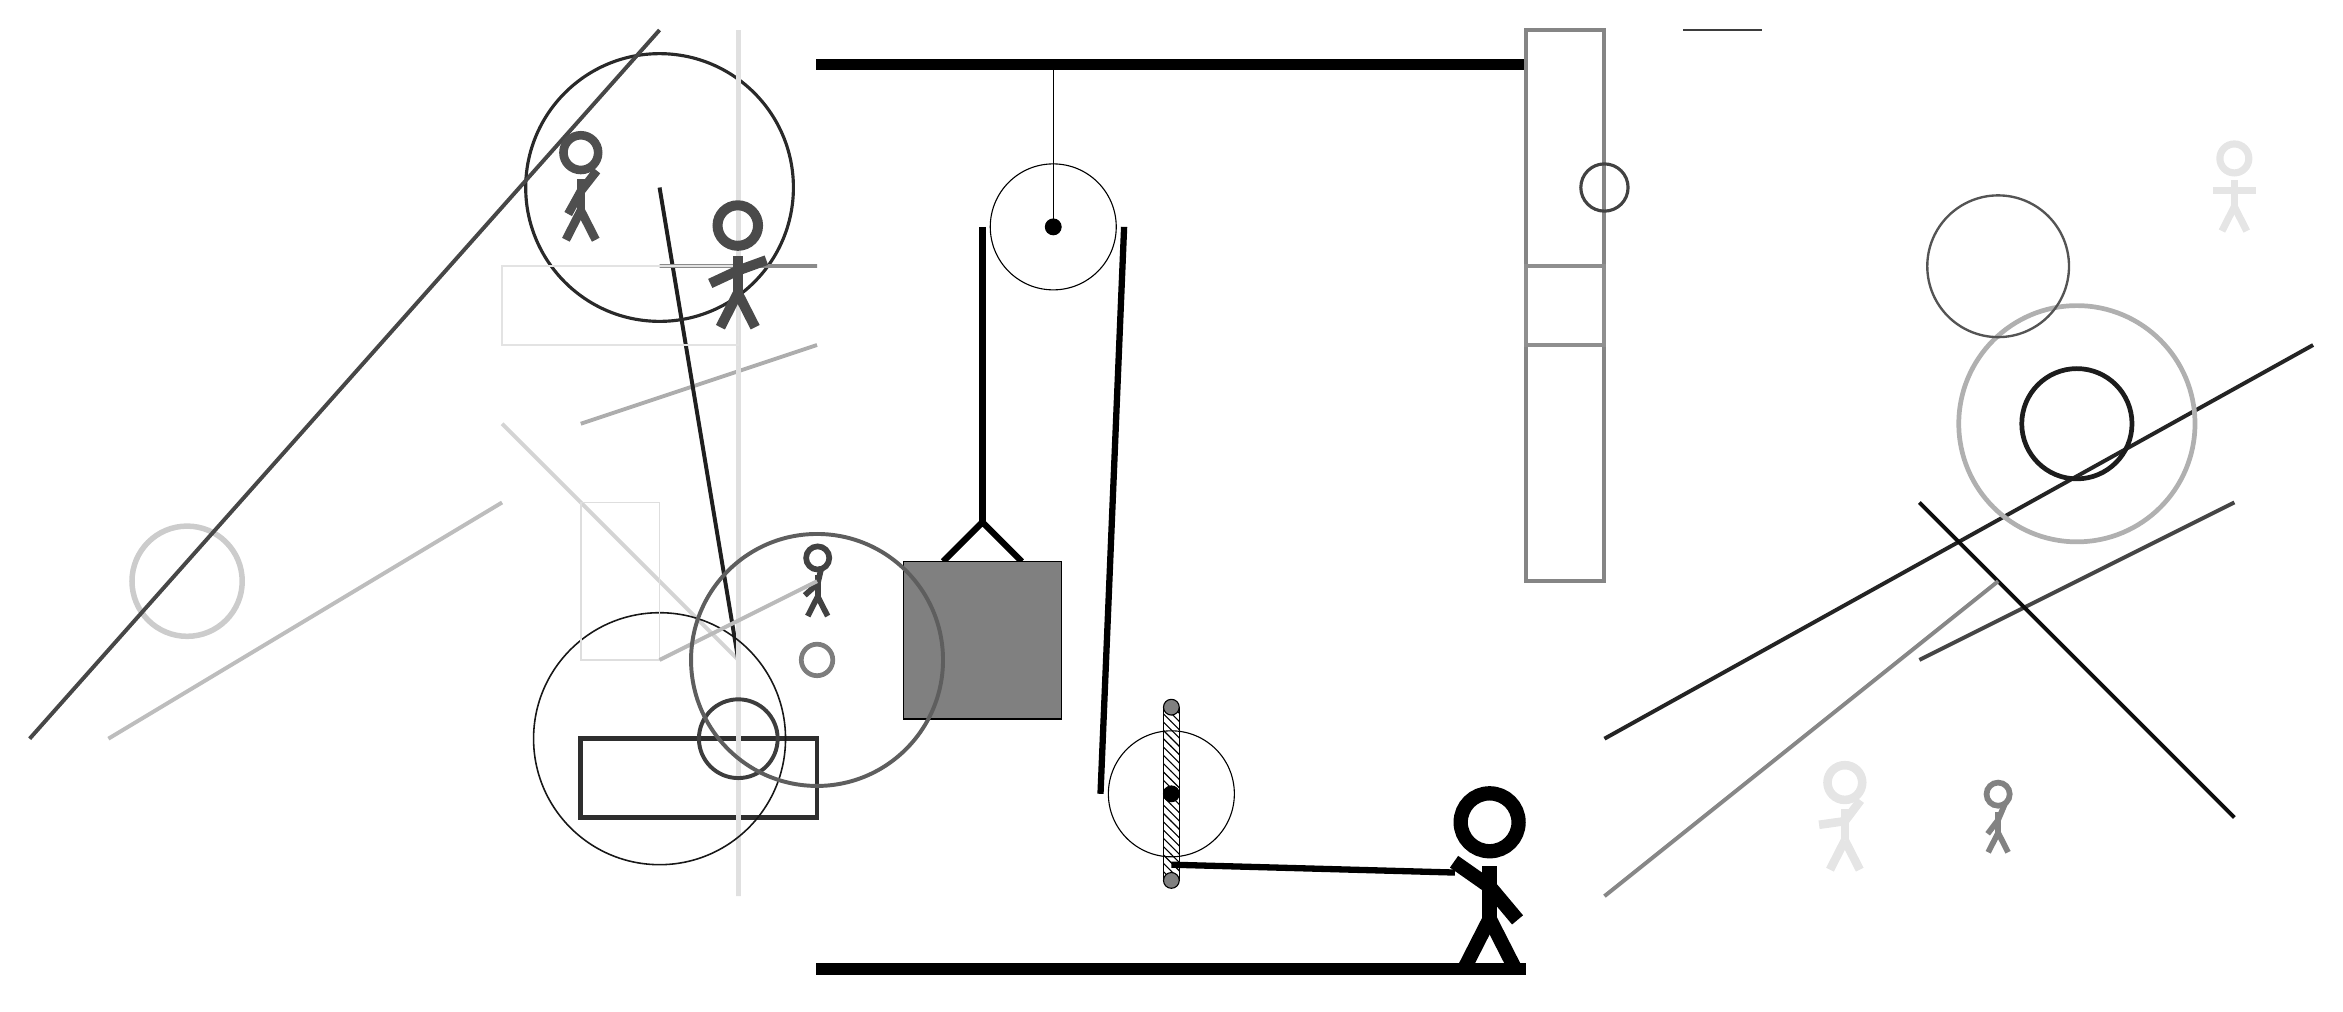
\begin{tikzpicture}
			%%%%% START %%%%%
			
			\draw[fill=black] (-2, 11.5) rectangle (7, 11.625);
			
			\draw (1, 9.5) circle (0.8);
			\draw[fill=black] (1, 9.5) circle (0.1);
			\draw (1, 11.5) -- (1, 9.5);
			
			\draw[fill=white](2.5, 2.3) circle (0.8);
			\draw[fill=black] (2.5, 2.3) circle (0.1);
			\draw[pattern=north west lines, pattern color=black] (2.4, 3.4) rectangle (2.6, 1.2);
			\draw[fill=black!50] (2.5, 3.4) circle (0.1);
			\draw[fill=black!50] (2.5, 1.2) circle (0.1);
			
			\draw[line width=0.8mm] (-0.4, 5.25) -- (0.1, 5.75) -- (0.6, 5.25);
			\draw[fill=black!50] (-0.9, 5.25) rectangle (1.1, 3.25);
			
			\draw[line width=0.8mm] (0.1, 9.5) -- (0.1, 5.75);
			\centerarc[line width=0.8mm](1, 9.5)(0:180:0.9);
			\draw[line width=0.8mm](1.9, 9.5) -- (1.6, 2.3);
			\centerarc[line width=0.8mm](2.5, 2.3)(180:270:0.9);
			\draw[line width=0.8mm](2.5, 1.4) -- (6.1, 1.3);
			
			\draw[line width=0.5mm, color=black!73](12, 4) -- (16, 6);
			
			\draw[line width=0.5mm, color=black!17](-3, 4) -- (-6, 7);
			\draw[line width=0.5mm, color=black!32](-2, 8) -- (-5, 7);
			\draw[line width=0.5mm, color=black!88](-4, 10) -- (-3, 4);
			\draw[line width=0.6mm, color=black!82] (-2, 2) rectangle (-5, 3);
			\draw[line width=0.2mm, color=black!76] (9, 12) rectangle (10, 12);
			
			\draw [line width=0.4mm, color=black!84](-4, 10) circle (1.7);
			
			\draw[line width=0.5mm, color=black!86](8, 3) -- (17, 8);
			\node[line width=0.5mm, color=black!10] at (11, 2) {\Strichmaxerl[6][8][53]};
			
			\draw[line width=0.5mm, color=black!46] (-4, 9) rectangle (-2, 9);
			
			\draw[line width=0.6mm, color=black!12] (-3, 1) rectangle (-3, 12);
			
			\draw[line width=0.5mm, color=black!26](-6, 6) -- (-11, 3);
			\draw [line width=0.5mm, color=black!76](-3, 3) circle (0.5);
			
			\draw[line width=0.5mm, color=black!95](12, 6) -- (16, 2);
			\node[line width=0.5mm, color=black!10] at (16, 10) {\Strichmaxerl[5][0][0]};
			\draw [line width=0.7mm, color=black!20](-10, 5) circle (0.7);
			\draw [line width=0.2mm, color=black!91](-4, 3) circle (1.6);
			
			\draw [line width=0.6mm, color=black!31](14, 7) circle (1.5);
			\draw[line width=0.5mm, color=black!72](-4, 12) -- (-12, 3);
			
			\draw[line width=0.5mm, color=black!47](8, 1) -- (13, 5);
			\draw [line width=0.3mm, color=black!67](13, 9) circle (0.9);
			
			\draw[line width=0.2mm, color=black!11] (-3, 8) rectangle (-6, 9);
			
			\draw[line width=0.5mm, color=black!48] (7, 12) rectangle (8, 5);
			\node[line width=0.5mm, color=black!71] at (-3, 9) {\Strichmaxerl[7][25][20]};
			\node[line width=0.6mm, color=black!74] at (-2, 5) {\Strichmaxerl[4][42][77]};
			
			\draw [line width=0.4mm, color=black!74](8, 10) circle (0.3);
			
			\draw [line width=0.6mm, color=black!89](14, 7) circle (0.7);
			\draw[line width=0.2mm, color=black!13] (-4, 6) rectangle (-5, 4);
			
			\draw[line width=0.5mm, color=black!27](-4, 4) -- (-2, 5);
			\node[line width=0.3mm, color=black!69] at (-5, 10) {\Strichmaxerl[6][61][52]};
			\draw [line width=0.5mm, color=black!63](-2, 4) circle (1.6);
			\draw[line width=0.5mm, color=black!44] (7, 9) rectangle (8, 8);
			\draw [line width=0.6mm, color=black!51](-2, 4) circle (0.2);
			
			\node[line width=0.6mm, color=black!49] at (13, 2) {\Strichmaxerl[4][53][67]};
			
			
			\node at (6.5, 1.2) {\Strichmaxerl[10][-35][-50]};
			
			\draw[fill=black] (-2, 0) rectangle (7, 0.15);
			
			%%%%% END %%%%%
		\end{tikzpicture}
	\end{figure}	
\end{document}